\documentclass{article}

% if you need to pass options to natbib, use, e.g.:
%     \PassOptionsToPackage{numbers, compress}{natbib}
% before loading neurips_2019

% ready for submission
% \usepackage{neurips_2019}

% to compile a preprint version, e.g., for submission to arXiv, add add the
% [preprint] option:
%     \usepackage[preprint]{neurips_2019}

% to compile a camera-ready version, add the [final] option, e.g.:
     \usepackage[final]{neurips_2019}

% to avoid loading the natbib package, add option nonatbib:
%     \usepackage[nonatbib]{neurips_2019}

\usepackage[utf8]{inputenc} % allow utf-8 input
\usepackage[T1]{fontenc}    % use 8-bit T1 fonts
\usepackage{hyperref}       % hyperlinks
\usepackage{url}            % simple URL typesetting
\usepackage{booktabs}       % professional-quality tables
\usepackage{amsfonts}       % blackboard math symbols
\usepackage{nicefrac}       % compact symbols for 1/2, etc.
\usepackage{microtype}      % microtypography

% My packages

\usepackage[mathscr]{euscript}
\usepackage{natbib}
\usepackage{graphicx}
\usepackage {tikz}
\usetikzlibrary {positioning}
\usepackage{amsthm}
\usepackage{amsmath}
\usepackage{amssymb}
\usepackage{dsfont}
\usepackage{hyperref}
\usepackage{stmaryrd }
\usepackage{csquotes}
\usepackage{wasysym}

\theoremstyle{plain}
\newtheorem{theorem}{Theorem}
\newtheorem{corollary}[theorem]{Corollary}
\newtheorem{lemma}[theorem]{Lemma}

\theoremstyle{definition}
\newtheorem{definition}{Definition}[section]
\newtheorem{example}{Example}[section]

\newcommand{\CI}{\mathrel{\text{\scalebox{1.07}{$\perp\mkern-10mu\perp$}}}}
\newcommand{\CII}{\mathrel{\text{\scalebox{1.07}{$\perp\mkern-10mu\perp\mkern-10mu\perp$}}}}
\newcommand{\RV}[1]{\ensuremath{\mathsf{#1}}}
\newcommand{\PA}[2]{\ensuremath{\text{Pa}_{#1}(#2)}}
\newcommand{\ND}[2]{\ensuremath{\text{ND}_{#1}(#2)}}
\newcommand{\CH}[2]{\ensuremath{\text{Ch}_{#1}(#2)}}
\newcommand{\DE}[2]{\ensuremath{\text{De}_{#1}(#2)}}

\newcommand\splitter[1]{%
\begin{tikzpicture}[scale=#1]
\draw (0,-1) -- (0,0);
\draw (0,0) to [bend right] (1,1);
\draw (0,0) to [bend left] (-1,1);

\end{tikzpicture}
}

\newcommand\stopper[1]{%
\begin{tikzpicture}[scale=#1]
\draw (0,-1) -- (0,0);
\node (E) at (0,0) {$\bigcdot$};

\end{tikzpicture}
}

\DeclareMathOperator*{\argmax}{arg\,max}
\DeclareMathOperator*{\argmin}{arg\,min}
\DeclareMathOperator*{\arginf}{arg\,inf}
\DeclareMathOperator*{\argsup}{arg\,sup}

\title{How to ask a causal question}

% The \author macro works with any number of authors. There are two commands
% used to separate the names and addresses of multiple authors: \And and \AND.
%
% Using \And between authors leaves it to LaTeX to determine where to break the
% lines. Using \AND forces a line break at that point. So, if LaTeX puts 3 of 4
% authors names on the first line, and the last on the second line, try using
% \AND instead of \And before the third author name.

\author{%
  David Johnston\thanks{Use footnote for providing further information
    about author (webpage, alternative address)---\emph{not} for acknowledging
    funding agencies.} \\
  College of Engineering and Computer Science\\
  Australian National University\\
  ACT, Australia 0200 \\
  \texttt{david.johnston1@anu.edu.au} \\
  % examples of more authors
   \And
  Cheng Soon Ong\\
  Data61\\
  % Address \\
  % \texttt{email} \\
   \AND
   Robert Williamson \\
   Data61 and College of Engineering and Computer Science\\
   Australian National University\\
  % Address \\
  % \texttt{email} \\
  % \And
  % Coauthor \\
  % Affiliation \\
  % Address \\
  % \texttt{email} \\
  % \And
  % Coauthor \\
  % Affiliation \\
  % Address \\
  % \texttt{email} \\
}


\begin{document}

\maketitle

\begin{abstract}
  The abstract paragraph should be indented \nicefrac{1}{2}~inch (3~picas) on
  both the left- and right-hand margins. Use 10~point type, with a vertical
  spacing (leading) of 11~points.  The word \textbf{Abstract} must be centered,
  bold, and in point size 12. Two line spaces precede the abstract. The abstract
  must be limited to one paragraph.
\end{abstract}

\section{Notation}

\begin{itemize}
    \item A subscript on a random variable $\RV{X}_i$ refers to its position in a sequence of (usually IID) random variables taking values in the same space
    \item A superscript on a random variable $\RV{X}^i$ marks it out as an element of a set of random variables that do not necessarily take values in the same space
    \item The notation $[N]$ refers to the set of natural numbers $\{0,...,N\}$
\end{itemize}

\section{Definitions}

\cheng{One sentence describing the difference between $E$ and $\mathcal{E}$. Explicitly say that you are using caligraphic letters to mean measures, e.g. $\mathcal{G}, \mathcal{H}$ below.}

\cheng{Generally, you need to define notation (instead of expecting the reader to infer from type signatures).}

\cheng{You need to clarify the distinction between measures and probability measures.}

Given two measureable sets $(E,\mathcal{E})$ and $(F,\mathcal{F})$, a \emph{Markov kernel} $K:E\to \Delta(\mathcal{F})$ is a map where
\begin{enumerate}
    \item The map $x\mapsto K(x;B)$ is $\mathcal{E}$-measurable for every $B\in\mathcal{F}$
    \item The map $B\mapsto K(x;B)$ is a probability measure on $(F,\mathcal{F})$ for every $x\in E$
\end{enumerate}

Abusing notation somewhat, we will write the set of Markov kernels of type $E\to \Delta(\mathcal{F})$ as $\Delta(\mathcal{F})^D$.

Two Markov kernels $K:E\to \Delta(\mathcal{F})$ and $K':E\to \Delta(\mathcal{F})$ are $\mu$-almost surely equivalent given $\mu\in \Delta(\mathcal{E})$ if
\begin{align}
    \int_A K(x;B) d\mu = \int_A K'(x;B) d\mu\qquad\forall A\in \mathcal{E}, B\in\mathcal{F}
\end{align}

Given $\mu\in \Delta(\mathcal{E})$ and a sub-$\sigma$-algebra $\mathcal{D}\subset\mathcal{E}$, there is a Markov kernel $\mu_{\mathcal{D}}:E\to\Delta(\mathcal{E})$ such that for $A\in\mathcal{E}$ and $B\in \mathcal{D}$, $\int_B \mu_{\RV{X}}(y;A) d\mu(y) = \mu(A\cap B)$. $\mu_{\mathcal{D}}$ is a \emph{conditional probability distribution} with respect to $\mathcal{D}$. Given a set of random variables $\mathbf{X}=\{\RV{X}^i\}_{i\in [N]}$ with domain $(E,\mathcal{E})$, $\mu_{\mathbf{X}}$ is a conditional probability distribution with respect to the $\sigma$-algebra generated by $\mathbf{X}$: $\sigma(\cup_{i\in[N]}\sigma(\mathcal{X}^i))$.

\cheng{$D$ not defined.}

\cheng{$\Delta$ not defined.}

\subsection{Operations with Markov kernels}

For the following, assume $K$ is a Markov kernel from $E\to \Delta(\mathcal{F})$, L is a Markov kernel $F\to \Delta(\mathcal{G})$, $\mu$ is a probability measure on $(E,\mathcal{E})$ and $f$ is a nonnegative measurable function $F\to \mathbb{F}$. More details can be found in Appendix \ref{app:markov_kernels}

\cheng{$\mathbb{F}$ needs clarification.}

The notation here borrows heavily from \cite{cinlar_probability_2011} and \cite{fong_causal_2013}.

\cheng{You need to write a small tutorial about Markov kernels, otherwise reader cannot follow.}

\subsubsection{Kernel products}

\cheng{Explicitly say that $KL$ is a product of kernels $K$ and $L$. Symmetric? Distributive? Similarly for all the other products.}

$KL$ is a Markov kernel $E\to \Delta(\mathcal{G})$ such that
\begin{align}
    KL(x;B):= \int_F K(x;dy) L(y;B),\qquad x\in E, B\in \mathcal{G}
\end{align}

$\mu K$ is a probability measure on $(F,\mathcal{F})$ such that
\begin{align}
    \mu K(B)=\int_E \mu(dx) K(x;B),\qquad B\in\mathcal{F}
\end{align}

\subsubsection{Special kernels and operations}


$I_E$ is the identify kernel $E\to \Delta(\mathcal{E})$ defined by $x\mapsto \delta_x$. It has the properties $\mu I_E=\mu$, $KI_F = K$, $I_E K = K$, $I_F f=f$.
=======
\cheng{Motivate why we need these special definitions. I think the kernels are special, but operations not.}

\cheng{Also teach the reader how to say the symbols $\splitter{0.15}, \stopper{0.15}$.}



Given some measurable function $g:E\to F$, the kernel $F_g:E\to \Delta(\mathcal{F})$ is defined by $x\mapsto \delta_{g(x)}$. It is easy to check that $F_g F_g = F_g$. For $\mu\in \Delta(\mathcal{E})$, the product $\mu F_g$ is the push forward measure $g_*\mu$. 

Given $\mu\in \Delta(\mathcal{E}$, $\mu\splitter{0.15}(I_E\otimes K)$ is a distribution in $\Delta(\mathcal{E}\otimes\mathcal{F})$ given by
\begin{align}
    \mu\splitter{0.15}(I_E\otimes K)(A\times B) = \int_A K(x;B) d\mu(x)\qquad \forall A\in \mathcal{E},B\in \mathcal{F}
\end{align}


Given a set of random variables $\{\RV{X}^i\}_{i\in[N]}$ with domain $(E,\mathcal{E})$,  $\mu\splitter{0.15}(\otimes_{i\in[N]} F_{\RV{X}^i})$ is the joint distribution the set.

\cheng{Reviewers are not going to be patient enough to sit through 2 pages of definitions. You need to motivate why you need so many spaces, measures, products, etc.}


\section{Causal Statistical Decision Problems}
\begin{table}[ht]
    \centering
\begin{tabular}{ |c|c|c| } 
 \hline
  & SDPs & CSDPs \\ 
 \hline
 State of the world & $\mathscr{H}$, hypothesis class & $\mathscr{T}$, causal theory \\ 
 Observations & $\RV{X}$ & $\RV{X}$ \\ 
 Decisions & $D$ & $D$ \\
 Known preferences & $\ell$, loss & $U$, pseudo-utility \\
 Derived preferences & $\ell$, loss & $L$, causal loss\\
 \hline
\end{tabular}
    \caption{Comparison of SDPs and CSDPs}
    \label{tab:sdp_cdp_comparison}
\end{table}

We develop causal statistical decision problems (CSDPs) as an extension of statistical decision problems (SDPs) where our preferences (i.e. utility or loss) are known less directly in former case. Following \citep{toutenburg_ferguson_1967}, we consider SDPs and causal statistical decision problems CSDPs to represent normal form two person games. The games represent at the most abstract level the options and possible payoffs available to the decision maker, and this representation allows us to compare the two types of problem. In their more detailed versions,  CSDPs and SDPs differ in their representation of the state of the world and in the type of function that represents preferences. These differences are summarised in Table \ref{tab:sdp_cdp_comparison}.

\begin{definition}[Normal form two person game]
A normal form game is a triple $\langle \mathscr{S}, A, L\rangle$ where $\mathscr{S}$ and $A$ are arbitrary sets and $L:\mathscr{S}\times A\to [0,\infty)$ is a loss function.

\end{definition}
The set $\mathscr{S}$ is a set of possible states that the environment may occupy and $A$ is a set of actions the decision maker may take. The decision maker seeks an action in $A$ that minimises the loss $L$. Generally there is no action that minimises the loss for all environment states. A minimax solution is an action that minimises the worst case loss: $a^*_{mm} = \argmin_{a\in A} [\sup_{s\in \mathscr{S}} L(s,a)]$.

If the set $\mathscr{S}$ is equipped with a $\sigma$-algebra $\mathcal{S}$ and a probability measure $\xi\in \Delta(\mathcal{S})$ which we will call a ``prior'', a Bayes solution minimizes the expected risk with respect to $\xi$: $a^*_{ba} = \argmin_{a\in A} \int_{\mathcal{S}} L(s,a) \xi(ds)$.

\begin{definition}[Admissible Action]
Given a normal form two person game $\langle \mathscr{S}, A, L\rangle$, an action $a\in A$ is strictly better than $a'\in A$ iff $L(s,a)\leq L(s,a')$ for all $s\in\mathscr{S}$ and $L(s_0,a)<L(s_0,a')$ for some $s_0\in \mathscr{S}$. If only the first holds, then $a$ is as good as $a'$. An admissible action is an action $a\in A$ such that there is no action strictly better than $A$.
\end{definition}

\begin{definition}[Complete Class]
A class $C$ of decisions is a complete class if for every $a\not\in C$ there is some $a'\in C$ that is strictly better than $a$.

A class $C$ is an essentially complete class if for every $a\not\in C$ there is some $a'\in C$ that is as good as $a$.
\end{definition}

\begin{definition}[Reduction]\label{def:red_sdp_CSDP}
A normal form two person game $\alpha = \langle \mathscr{S}^\alpha, A, L^\alpha\rangle$ can be reduced to a different game sharing the same action set $\beta = \langle \mathscr{S}^\beta, A, L^\beta \rangle$ if there is a surjective function $g:\mathscr{S}^\alpha\to \mathscr{S}^\beta$ such that for every $a\in A$, $s\in \mathscr{S}^\alpha$, $L^\alpha(s,a) = L^\beta(g(s),a)$.
\end{definition}

Because CSDPs and SDPs posit states of nature of different types, they cannot represent exactly the same game. Reduction is a notion that allows us to say tht the game represented by a CSDP and an SDP are ``essentially'' the same. Reduction preserves the important properties of admissibility and completeness as shown in Appendix \ref{app:csdps}.

A statistical decision problem represents a normal form two-person game where the available actions are \emph{decision functions} that output a decision given data, the states of the environment are associated with probability measures on some measurable space and we assume a loss expressing preferences over decisions and states is known.

\begin{definition}[Statistical Decision Problem]
A statistical decision problem (SDP) is defined by a tuple $\langle (\mathscr{H},(E,\mathcal{E}), \RV{X}), (D,\mathcal{D}), \ell\rangle$. $\mathscr{H}\subset\Delta(\mathcal{E})$ is a hypothesis class representing possible states of the environment, $D$ is the set of available decisions, $\RV{X}:(E,\mathcal{E})\to (X,\mathcal{X})$ is a random variable representing the information available for the statistician to make a decision and $\ell:\mathcal{H}\times D\to [0,\infty)$ is a loss function.

Denote by $\mathscr{J}$ the set of decision kernels $X\to \Delta(\mathcal{D})$. Recall that $\mu F_{\RV{X}}(A)=\mu(\RV{X}^{-1}(A))$. For $J\in \mathscr{J}$ and $\mu\in \mathcal{H}$, the risk $R:\mathscr{J}\times\mathscr{H}\to [0,\infty)$ is defined as $R(J,\mu) = \int_D \ell(\mu,y) \mu F_{\RV{X}} J(dy)$.

Denoting by $\mathscr{J}$  the set of kernels $X\to \Delta(\mathcal{D})$, the triple $\langle \mathscr{H}, \mathscr{J}, R\rangle$ forms a two player normal form game.
\end{definition}


The loss function $\ell$ expresses preferences over (state, decision) pairs. However, it may be the case that our preferences don't naturally apply directly to such pairs. For a doctor deciding whether to prescribe a treatment to a patient, it is clear that this patient being healthy in the future is preferable to them being sick. This motivates the definition of a causal statistical decision problem, utilising a preferences defined over outcomes rather than (state, decision) pairs. In order to compute the loss associated with a decision a map from decisions to outcomes is required, which we term a \emph{consequence}.

\begin{definition}[Consequences]
Given a measurable outcome space $(F,\mathcal{F})$ and a measurable decision space $(D,\mathcal{D})$, a Markov kernel $\kappa:D \to \Delta(\mathcal{F})$ is a \emph{consequence mapping}, or just a consequence for short.
\end{definition}

\begin{definition}[Causal state]
Given a consequence $\kappa:D\to \Delta(\mathcal{F})$, a measurable observation space $(E,\mathcal{E})$ and some distribution $\mu\in \Delta(\mathcal{E})$, the pair $\tau:=(\kappa,\mu)$ is a \emph{causal state} on $D, E$ and $F$. We refer to $\kappa$ as the consequence and $\mu$ as the observed state.
\end{definition}

\begin{definition}[Causal Theory]\label{def:causal_theory}
A causal theory $\mathscr{T}$ is a set of causal states sharing the same decision, observation and outcome spaces.
\end{definition}

\cheng{You need to define the different uses of ``utility''. E.g. utility, pseudo-utility, ordinary utility, generalized utility, normal utility. Or perhaps be more careful with your usage.}

\cheng{The change from loss $\ell$ to $(U,F)$ is a surprising, so you need to explain why you need to do so.}

\cheng{The following definition is too long. Defines too many things.}

\begin{definition}[Causal Statistical Decision Problem]\label{def:CSDP}
A causal statistical decision problem (CSDP) is a tuple $\langle (\mathscr{T}, (E,\mathcal{E}) \RV{X}), (D,\mathcal{D}), (U,(F,\mathcal{F})) \rangle$. $\mathscr{T}$ is a causal theory on $D, E$ and $F$, $D$ is the decision set, $\RV{X}:(E,\mathcal{E})\to (X,\mathcal{X})$ is a random variable representing the given information and $U:\Delta(\mathcal{F}\otimes \mathcal{D})\to \mathbb{R}$ is a pseudo-utility expressing preference over joint distributions of decisions and outcomes which we assume is bounded above.

From the pseudo-utility $U$ we can define a loss $L:\mathscr{T}\times\Delta(\mathcal{D})\to [0,\infty]$ by
\begin{align}
    L((\kappa,\mu),\gamma) := \sup_{\gamma'\in\Delta(\mathcal{D})} U(\gamma'\splitter{0.15}(I_D\otimes \kappa)) - U(\gamma\splitter{0.15}(I_D\otimes \kappa))\label{eq:canonical_loss}
\end{align}
For $(\kappa,\mu)\in \mathscr{T}$ and $\gamma\in \Delta(\mathcal{D})$. This is well defined wherever $U$ is bounded above. Note that $L$ does not depend on the data generating distribution $\mu$; henceforth we will suppress this argument and write $L(\kappa,\gamma):= L((\kappa,\mu),\gamma)$.

Given a decision function $J\in\mathscr{J}$ and $(\kappa,\mu)\in \mathscr{T}$, we define the risk $R:\mathscr{J}\times \mathscr{T}\to [0,\infty)$ by $R(J,\kappa,\mu) := L(\kappa,\mu F_{\RV{X}} J)$.

The triple $\langle \mathscr{T}, \mathscr{J}, R\rangle$ is a normal form two person game.

If there exists some measurable $u:F\times D\to \mathbb{R}$ such that for all $\xi\in \Delta(\mathcal{F}\otimes\mathcal{D})$, $U(\xi)=\mathbb{E}_{\xi}[u]$ then we call $u$ an ordinary utility and by extension $U$ an ordinary pseudo-utility.

An ordinary utility induces a loss $L(\kappa,\gamma) = \mathbb{E}_{\gamma}[l^\kappa]$
where $l^\kappa:D\to [0,\infty)$ is defined by
\begin{align}
    l^\kappa(d) := \sup_{\gamma'\in \Delta(\mathcal{D})} \mathbb{E}_{\gamma'\splitter{0.08}(I_D\otimes \kappa)}[u] - \mathbb{E}_{\kappa(d;\cdot)}[u(\cdot,d)]\label{eq:induced_l}
\end{align}
\end{definition}

\cheng{Create a table that summarises the similarities and differences between the two decision problems.}

Reduction from a CSDP to an ordinary SDP is sufficient to import results from statistical decision theory such as Theorem \ref{th:complete_class}.

\cheng{Explain why complete class is important.}

\begin{theorem}[Complete class theorem (CSDP)]\label{th:complete_class}
Given an CSDP $\alpha:=\langle (\mathscr{T},E),D,\RV{X},U\rangle$ with risk $R$, if there is a reduction to an SDP $\beta:=\langle (\mathscr{H},F),D,\RV{Y},\ell \rangle$ with risk $R'$ such that $|\mathscr{H}|<\infty$ and $\inf_{J\in\mathscr{J},\mu\in\mathscr{H}} R'(J,\mu)<-\infty$, then the set of all Bayes decision functions is a complete class for $\beta$ and the set of all admissible Bayes decision functions is a minimal complete class for $\beta$.
\end{theorem}

\begin{proof}
This follows from Lemmas \ref{cor:red_comp} and \ref{lem:IB_rule}. See appendix \ref{app:csdps}.
\end{proof}

Any statistical decision problem can be reduced to a CSDP featuring a causal theory where decisions have no effect.

\cheng{Justify the choice of word ``reduce''.}


\begin{theorem}\label{th:sdp_to_CSDP}
Every SDP $\langle (\mathscr{H},E,\RV{X}),D,\ell\rangle$ can be reduced to a CSDP.
\end{theorem}
\begin{proof}
Choose a theory that matches every probability measure $\mu\in\Delta(\mathcal{E})$ with a consequence map that itself always yields $\mu$. Then construct a utility $U$ that induces an identical risk. See Appendix \ref{app:csdps}.
\end{proof}

The pseudo-utility $U$ enables Theorem \ref{th:sdp_to_CSDP}. A reduction is sometimes possible to an CSDP featuring an ordinary utility with a nontrivial theory, but whether this is always possible remains an open question.

A CSDP cannot, in general, be reduced to a statistical decision problem - for example, if we choose the utililty to be the variance of some random variable we may be able to achieve higher utility through a randomised decision than any nonrandomised decision under conditions where a regular SDP cannot have this property (see Example \ref{ex:ired_csdp} in Appendix \ref{app:csdps}). It is an open question whether this reduction is generally possible if the problem features a normal utility.

Theorem \ref{th:red_CSDP} reduces a CSDP to a SDP by associating each pair $(\mu,\kappa)$ in the causal theory with a distribution over $E\times F\times D$. This may be possible by finding a distribution on the product space for which $\mu$ is a marginal probability and $\kappa$ is a conditional distribution, but this is not necessary.

\begin{theorem}\label{th:red_CSDP}
Given a CSDP $\beta=\langle (\mathscr{T},E,\RV{X}),D,(U,F)\rangle$ where $U$ is an ordinary pseudo-utility, let $\mathscr{K}=\{\kappa|(\kappa,\mu)\in \mathscr{T}\}$ be the set of consequences. $\beta$ is reducible to a statistical decision problem on the measurable space $(E\times F\times D,\mathcal{E}\otimes \mathcal{F}\otimes \mathcal{D})$ if there is some surjective map $m:\Delta(\mathcal{F}\otimes\mathcal{D})\to \mathscr{K}$.
\end{theorem}

\begin{proof}
We construct the map $h$ based on the map $m$ and show that, given an ordinary utility $U$, it is possible to construct a loss $\ell$ such that the resulting SDP features the same risk assignments as the original CSDP. See Appendix \ref{app:csdps}.
\end{proof}

\begin{corollary}\label{cor:card_reduc}
If the cardinality of $\Delta(\mathcal{F}\otimes\mathcal{D})$ is at least as large as the cardinality of the set of Markov kernels $D\to \Delta(\mathcal{F})$ then an CSDP with an ordinary utility can always be reduced to a SDP.
\end{corollary}

\begin{proof}
This follows from Theorem \ref{th:red_CSDP} and the definition of cardinality.
\end{proof}

A major open question, then, is if $(E,\mathcal{E})$ and $(D,\mathcal{D})$ are standard measurable spaces, the conditions for Corollary \ref{cor:card_reduc} hold in general. Corollary \ref{cor:CSDP_to_sdp} shows that the reduction can be made in general if $D$ is a denumerable set.

\begin{corollary}\label{cor:CSDP_to_sdp}
A CSDP $\langle (\mathscr{T},(E,\mathcal{E}),\RV{X}),(D,\mathcal{D}),(U,(F,\mathcal{F}))\rangle$ where $D$ is a denumerable set and $U$ is an ordinary pseudo-utility can be reduced to a statistical decision problem.
\end{corollary}

\begin{proof}
Take some probability measure $\pi\in \Delta(\mathcal{D})$ such that $\pi(\{y\})>0$ for all $y\in D$. Such a $\pi$ exists by the denumerability of $\mathcal{D}$. The map $m:\Delta(\mathcal{F}\otimes\mathcal{D})\to \mathscr{K}$ given by $m(\xi)(y;A) := \frac{\xi(A\times\{y\})}{\pi(\{y\})}$ is surjective. The result follows from Theorem \ref{th:red_CSDP}.
\end{proof}

This reduction is not particularly practically useful, but it is sufficient to lift results such as Theorem \ref{th:complete_class} from the theory of statistical decision functions.

\section{Causal Bayesian Networks}

A causal Bayesian network is an example of an identifiable causal theory. Given a measurable space $(X,\mathcal{X})$ where $X=\times_{i\in [N]} X^i$, a decision space $D = \times_{i\in [N]} X^i\cup\{*\}$ and a causal graph $\mathcal{G}$ over nodes $\mathbf{V}=\{V^i|i\in [N]\}$, the graph $\mathcal{G}$ maps each probability distribution $\mu\in \Delta(\mathcal{X})$ to a unique consequence $D\to \Delta(\mathcal{X})$.

The CBN convention is to call the elements of the decision space $D$ ``interventions'' and denote then with $P(\cdot|do(\cdot\cdot))$ notation. In the first definition below, we instead denote interventions with indices on the probability distribution, and introduce the special $*$ object to denote a passive intervention.

\begin{definition}[Causal Bayesian Network]\label{def:CBN}
The definition here follows \cite{pearl_causality:_2009}.

Consider a directed acyclic graph $\mathcal{G}$ with nodes $\mathbf{X}=\{\RV{X}^i|i\in [N]\}$, a measurable space $(E,\mathcal{E})$ and a set of random variables $\RV{X}^i:E\to X^i$ and let $X=\times_{i\in[N]} X^i$. For each $x\in \times_{i\in [N]} X^i\cup \{*\}$ suppose we have an \emph{interventional distribution} $P^{x}\in \Delta(\mathcal{E})$, and let the set of all such distributions be denoted $\mathbf{P}^{X\cup\{*\}}$. Let $P^*$ be the passive distribution given by the intervention $x = (*,...,*)$.

Given any $x\in X\cup\{*\}$ let $S(x)\subset[N]$ be the set of all indices $i$ such that $x^i\neq *$. The graph $\mathcal{G}$ is a causal Bayesian network compatible with $\mathbf{P}^{X\cup\{*\}}$ iff for all $x\in X$ and $S(x)\subset [N]$:
\begin{enumerate}
    \item $P^{x}_{\RV{X}}$ is compatible with $\mathcal{G}$ for all $x\in \cup_{i\in [N]} X^i\cup \{*\}$
    \item $P^x_{\RV{X}}(\RV{X}^{S(x)})=\delta_{x^{S(x)}}(\RV{X}^{S(x)})$
    \item For $i\in S^C$, $P^x_{\RV{X}}(\RV{X}^i|\PA{\mathcal{G}}{\RV{X}^i})=P^*_\RV{X}(\RV{X}^i|\PA{\mathcal{G}}{\RV{X}^i})$, $P^x$-almost surely
\end{enumerate}
\end{definition}

The above three conditions are sufficient that, given some graph $\mathcal{G}$ and $P^*_{\RV{X}}\in \Delta(\mathcal{X})$, one obtains a unique set of interventional distributions $\mathbf{P}_{\mathcal{G}}^{X\cup\{*\}}$ (this follows from the truncated factorisation property given by \cite{pearl_causality:_2009}). Identifying the decision set $D$ with $\times_{i\in [N]} X^i\cup\{*\}$, note that the map $\kappa^P_\mathcal{G}:D\to \Delta(\mathcal{X})$ given by $d\mapsto P^d_{\mathcal{G}}$ looks like a consequence map, which in fact it is (as established by Theorem \ref{th:cbn_MK}). The set of pairs $\{(P^*_{\RV{X}}, \kappa^P_\mathcal{G})|P^*_{\RV{X}}\in \Delta(\mathcal{X})\}$ is then a causal theory $\mathscr{T}_\mathcal{G}$.

\begin{theorem}\label{th:cbn_MK}
Given a graph $\mathcal{G}$, a measurable set $(E,\mathcal{E})$ and a decision set $D=\times_{i\in [N]} X^i\cup\{*\}$, let $P^x\in \Delta(\mathcal{E})$ be an interventional distribution compatible with $\mathcal{G}$ as defined in Definition \ref{def:CBN}. 

Then the map $\kappa_{\mathcal{G}}:D\to \Delta(\mathcal{X})$ given by $x\mapsto P^x$ is a Markov kernel.
\end{theorem}

The proof is given in Appendix \ref{app:cbn_ct}.

\subsection{Extending the theory induced by a CBN}

The causal theory associated with a given graph $\mathcal{G}$ is in general incomplete in that it does not associate a consequence with some distributions on $\Delta(\mathcal{X})$. In particular, if certain conditional independences are implied by $\mathcal{G}$, then probability distributions for which these conditional independences do not hold do not appear in the associated causal theory - only \emph{compatible} distributions are represented. This follows from condition 1 of Definition \ref{def:CBN}. While a theory doesn't have to feature a causal state for every possible distribution, it usually isn't reasonable to assume \emph{a priori} that certain conditional independences hold. In this case, it is necessary to extend the causal theory associated with $\mathcal{G}$ to cover distributions that are incompatible with $\mathcal{G}$.

The choice of how to extend the theory can be important. For discrete and jointly Gaussian distributions, conditional independences are associated with lower dimensional subspaces of the set of distributions\cite{meek_strong_1995}. Given causal theory $\mathscr{T}\subset$ and a $\sigma$-algebra $\mathcal{T}$, if we have a prior $\xi\in \Delta(\mathscr{H}\times \mathscr{K})$ such that the marginal $P^\xi(A)$ for $A\in \Delta(\mathscr{H})$ admits a density $P^\xi(A) = \int_A p^\xi(x)dx$ then this prior will assign 0 weight to any subset of $\mathscr{T}$ for which some conditional independence holds, and so for any $\mathcal{G}$ which is not fully connected the Bayes risk of any decision function $J$ is determined entirely by the extension of $\mathscr{T}$ to the set of distributions incompatible with $\mathcal{G}$.

An example follows. Suppose we have the following graph $\mathcal{G}$:

\begin{figure}
    \centering
     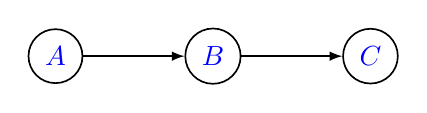
\begin{tikzpicture}[-latex,auto ,node distance =1 cm and 2cm ,on grid ,
    semithick ,
    vb/.style ={ circle ,top color =white , 
    draw , text=blue , minimum width =0.6 cm},
    kernel/.style={rectangle,draw}
    ]

    \node[vb] (A) {$A$};
    \node[vb] (B) [right = of A] {$B$};
    \node[vb] (C) [right = of B] {$C$};
    \draw (A) -- (B);
    \draw (B) -- (C);
    \end{tikzpicture}
    \caption{Simple causal Bayesian network $\mathcal{G}$}
    \label{fig:simple_cbn}
\end{figure}

Associated with this graph is the sample space $(E,\mathcal{E})=(\{0,1\}^3,\mathscr{P}(\{0,1\}^3)$ where $\mathscr{P}$ denotes the power set, and random variables $\RV{A},\RV{B}$ and $\RV{C}$ taking values in $\{0,1\}$. The set of possible distributions $\Delta(\mathcal{E})$ can be identified with the probability simplex in $\mathbb{R}^8$. For simplicity, suppose that only $A$ can be intervened on; that is, the decision space $D=A\cup\{*\}$ with the decision $\RV{D}_A=x$ for $x\in A$ having the usual interpretation as a hard intervention on $A$. We could alternatively assign infinite costs to interventions on $B$ and $C$, but this adds unnecessary complexity.

$\mathcal{G}$ implies $\RV{A}\CI \RV{C} | \RV{B}$. We have a theory $\mathscr{T}_{\mathcal{G}}$ associated with the graph $\mathcal{G}$ containing the state
\begin{align}
    (\nu,x\mapsto P^\nu(\RV{B}|\RV{A}=x) ) \label{eq:ocbn}
\end{align}
for every compatible $\nu$ . 

Consider two options for extending this to distributions $\nu$ incompatible with $\mathcal{G}$:
\begin{itemize}
    \item $\mathscr{T}_{\mathcal{G}}'$ assigns the causal states given by the union over all DAGs on the set of nodes $\{A, B, C\}$
    \item $\mathscr{T}_{\mathcal{G}}^\square$ assigns the causal states given by the union over all supergraphs of $\mathcal{G}$ on $\{A, B, C\}$
    \item $\mathscr{T}_{\mathcal{G}}^\circ$ assigns the causal states given by $\mathcal{G}$ and ignores the inconsistency of $\nu$
\end{itemize}

In the first theory, for every DAG featuring $A\to B$ there is a DAG featuring $B\to A$; in addition, there are a number of DAGs with no arrow between $A$ and $B$. Therefore any prior $\xi$ that admits a density over $\Delta(\mathcal{E})$ and assigns equal weight to each causal state in $\mathcal{T}$ featuring the same distribution will generate a posterior that assigns a weight of more than 0.5 to the possibility that the marginal distribution of $\RV{B}$ is independent of whatever decision $\RV{D}_A$ is chosen. This remains true even if the observed data consist of a very large number of IID observations distributed according to some $\pi$ for which it is indeed holds that $\RV{A} \CI_\pi \RV{C} | \RV{B}$.

The second theory, on the other hand, yields a set consequences that are ``close'' to the consequence given by the original graph $\mathcal{G}$ provided the distribution $\mu$ is sufficiently ``close'' to a distribution $\nu$ for which $\RV{A} \CI_\nu \RV{C} | \RV{B}$. Note that, marginalising over $\RV{A}$ and $\RV{C}$ and ignoring the passive action, the theory $\mathscr{T}^\square_{\mathcal{G}}$ associates two consequences with every incompatible $\mu$:
\begin{align}
    &(\mu,x\mapsto P^\mu(\RV{B}|\RV{A}=x) )\label{eq:cbn_s1}\\
    &(\mu,x \mapsto \sum_c P^\mu(\RV{B}|\RV{A}=x,\RV{C}=c)P^\mu(\RV{C}=c)) \label{eq:cbn_s2}
\end{align}

Note that \ref{eq:cbn_s1} matches the pattern for states in the original graph \ref{eq:ocbn}. Define the consequences $\kappa^\circ := x\mapsto P^\mu(\RV{B}|\RV{A}=x)$ and $\kappa^\square:= x \mapsto \sum_c P^\mu(\RV{B}|\RV{A}=x,\RV{C}=c)P^\mu(\RV{C}=c))$, leaving the $\mu$-dependence implicit.

Consider some $\mu$ for which $\RV{A} \CI_\mu \RV{C} | \RV{B}$ holds approximately. That is, for some $\epsilon>0$
\begin{align}
    \left|\sum_c P^\mu(\RV{B}|\RV{A}=x,\RV{C}=c)P^\mu(\RV{C}=c)-P^\mu(B|A=x)\right| &< \epsilon \label{eq:app_ci}
\end{align}

Suppose that we have some loss such that $L(\rho)= \mathbb{E}_\rho[\RV{B}] + k$. Noting that $\mathscr{T}^\circ_\mathcal{G}$ and $\mathscr{T}^\square_\mathcal{G}$ agree on $\kappa^\circ$, we can bound the disagreement between the two theories with
\begin{align}
    |R(J,\kappa^\square,\mu) - R(J,\kappa^\circ,\mu)| &=  \left|\mathbb{E}_{\mu J \kappa^\square} [\RV{B}] - \mathbb{E}_{\mu J \kappa^\circ} [\RV{B}]\right|\\
        &\leq \max_x \left|\sum_c P^\mu(\RV{B}|\RV{A}=x,\RV{C}=c)P^\mu(\RV{C}=c)-P^\mu(B|A=x) \right|\\
        &< \epsilon
\end{align}

The stipulation that the prior $\xi$ was such that the marginal distribution over $\Delta(\mathcal{E})$ admitted a density may be controversial. It is consistent with the notion that ``there are no true parametric zeros'' endorsed by many statisticians (for example  \cite{gelman_bayesian_2010,meehl_theory-testing_1967,berkson_difficulties_1938}). Furthermore, if conditional independences rarely hold precisely, then learners based on the theory $\mathscr{T}_{\mathcal{G}}'$ may usually converge to a state of skepticism even given a prior that assigns nonzero weight to the set of compatible probability distributions because the data are usually drawn from a distribution from which this independence does not hold.

\textbf{TODO (maybe)} A useful property to consider of causal theories is whether determining the data generating distribution $\mu$ is ``close'' to $\mu_0$ implies that the risk is ``close'' to $R(J,\mu_0,\kappa_0)$ for all $(\mu_0,\kappa_0)$ in $\mathscr{T}$. One has to choose a reasonable notion of closeness. There are possible results in the spirit of the example above for Bayesian networks.

\section{Potential Outcomes}

\textbf{Todo: } This story could be made stronger starting from the proposition that using PO or anything else, you still need to rate the desirability of available decisisons somehow.

Potential outcomes provide an alternative means to discuss causal effects. The standard setup posits a joint distribution between observed data $\RV{X}$, a treatment $\RV{Z}$ taking values in $[N]$ and several ``potential outcomes'' $\RV{X}_i$, $i\in [N]\setminus\{0\}$. At a minimum, the consistency condition is usually asserted (\cite{richardson2013single}): $\RV{Z}=i$ implies $\RV{X}_i=\RV{X}$. 

We modify this setup somewhat in order to analyse it in terms of a causal theory. We believe these choices are reasonable, but there is an element of interpretation involved here. For clarity every variable gets a subscript and $\RV{X}_{ob}$, $\RV{Z}_{ob}$ are random variables representing outcomes and treatments in the observed data. $\RV{X}_i, \RV{Z}_i$, $i\geq 0$ are random variables representing outcomes and treatments in consequence of choosing a decision $\RV{D}=i$ deterministically. Note that we do not necessarily have a ``passive decision'' as we did with CBNs. Finally, we work with a slightly weaker ``almost certain consistency'':

\begin{align}
    P(\RV{X}_i,\RV{X}_{ob}|\RV{Z}_{ob}=i,\RV{Z}_i=i)=\mathds{1}_{\RV{X}_{ob}=\RV{X}_i} \qquad\text{ with probabiliy 1}\label{eq:consistency}
\end{align}

Conditioning on $\RV{Z}_i=i$ is redundant under the usual assumption that $P(\RV{Z}_i) = \delta_i(\RV{Z}_i)$.

While there appears to be a natural identification of ``potential outcomes'' with consequences, observed data with observed state and treatments with decisions in a causal theory, it is usually not possible to represent a joint distribution obeying Condition \ref{eq:consistency} with a causal theory. Take the spaces $D,X,Z=\{0,1\}$ and suppose we have a causal theory $\mathscr{T}$ consisting of pairs $(\kappa,\mu)$ where $\mu\in\Delta(\mathcal{X}\otimes\mathcal{Z})$ and $\kappa$ is a Markov kernel from $D\to \Delta(\mathcal{X}\otimes\mathcal{Z})$. To construct a joint distribution between $\RV{X}_{ob}$ and $\RV{X}_i$ for $i\in \{0,1\}$ we take some deterministic decision function $J_i:X\times Z\to \Delta(\mathcal{D})$ where $J_i:(x,z;d)\mapsto \delta_i(d)$. For $A,C\in \Delta(\mathcal{X}\otimes\mathcal{Z})$, $B\in \Delta(\mathcal{D})$ we compose the objects as 
\begin{align}
    \xi(A\times B\times C) =  \int_B \int_A  \kappa(y; C) \delta_i(dy) \mu(dx\times dz)
\end{align}

For $\alpha\in\{ob,0,1\}$ take random variables $\RV{X}_\alpha:(X\times Z)^2\times D\to X$, $\RV{Z}_\alpha:(X\times Z)^2\times D\to X$ and $\RV{D}:(X\times Z)^2\times D\to D$ defined by projections $\RV{X}_\alpha:((x_{ob},z_{ob}),(x_i,z_i),d)\mapsto x_\alpha$, $\RV{Z}_\alpha$ similarly and $\RV{D}:((x_{ob},z_{ob}),(x_i,z_i),d)\mapsto d$. It is then straightforward to show that $(x,z,d))\mapsto \kappa(d; C)$ is a version of the conditional probability $P^\xi(\RV{X}_i|\RV{D},\RV{X}_{ob},\RV{Z}_{ob})$, which implies 
\begin{align}
    \RV{X}_i&\CI_\xi \RV{X}_{ob}|\RV{D}, \RV{Z}_{ob}
\end{align}
For any choice of $J_i,\mu,\kappa$. Noting that $J_i$ is deterministic, we also have
\begin{align}
    \RV{X}_i&\CI_\xi \RV{X}_{ob}|\RV{Z}_{ob} \label{eq:decision_d_sep}
\end{align}
Conditions \ref{eq:consistency} and \ref{eq:decision_d_sep} can hold simultaneously only if $\RV{X}_i$ and $\RV{X}_{ob}$ are deterministic conditional on $\RV{Z}_{ob}$. This is usually not the case.

In order to facilitate nontrival joint distributions between obsevations and potential outcomes, we introduce a \emph{generalised consequence}:

\begin{definition}[Generalised consequence]
Given a measurable consequence space $(F,\mathcal{F})$, a sample space $(E,\mathcal{E})$ and a measurable decision set $(D,\mathcal{D})$, a Markov kernel $\kappa:D\times E \to \Delta(\mathcal{F})$ is a generalised consequence.
\end{definition}

\begin{definition}[Generalised causal theory]
A generalised causal theory is the analogue of a causal theory with the consequence replaced by a generalised consequence.
\end{definition}

Given $D,X,Z$ as before, we provide an explicit construction respecting \ref{eq:consistency}. Here, for convenience, we identify $E=F=X\times Z$. For $x\in X$, $z\in Z$, $d\in D$ and $G\in \mathcal{X}$, $H\in \mathcal{Z}$ consider the kernel

\begin{align}
    \iota: (d,x,z;G\times H) \mapsto \delta_d(H)(\delta_z(H) \delta_x(G) + (1-\delta_z(H)) \iota'(d,x,z;G))
\end{align}

Where $\iota'$ is an arbitrary Markov kernel $D\times X\times Z\to \Delta(\mathcal{X}\otimes\mathcal{Z})$. It is straightforward to check that $\iota$ is a Markov kernel. Take the Consider the distribution given by
\begin{align}
    \zeta (A\times B\times C) =  \int_B \int_A  \iota(y,x,z; C) \delta_i(dy) \mu(dx\times dz)
\end{align}
And random variables $\RV{X}_i$, $\RV{Z}_i$ and $\RV{D}$ as before. Then
\begin{align}
    P^\zeta(\RV{X}_i=j,\RV{X}_{ob}=k|\RV{Z}_{ob}=i)P^\zeta(\RV{Z}_{ob}=i) &= \sum_{m,n} \iota(n,k,i;\{j,m\}) \delta_i(\{n\}) \mu(k,i)\\
     &= \sum_{m,n} \delta_n(m)[\delta_i(m) \delta_k(j) + (1-\delta_i(m))\iota'(n,k,i;\{j,m\})]\delta_i(\{n\}) \mu(k,i)\\
     &= \delta_k(j) \mu(k,i)
\end{align}

Which implies \ref{eq:consistency}.

\subsection{Causal Theories and Generalised Causal Theories}


A generalised causal decision problem is a causal decision problem featuring a generalised causal theory and a loss $L:\Delta(\mathcal{E}\otimes\mathcal{D}\otimes\mathcal{F})\to[0,\infty]$. There is a straightforward identification of causal theories with generalised causal theories, befitting the name. We might also ask when the extra structure of a generalised causal decision problem is needed.

Given an ordinary consequence $\kappa:D\to \Delta(\mathcal{F})$, we can trivially construct a generalised consequence $\iota:(d,e;A)\mapsto \kappa(d;A)$. In addition, given a loss $L:\Delta(\mathcal{D}\otimes\mathcal{F})\to[0,\infty]$ we can construct $L':\Delta(\mathcal{E}\otimes \mathcal{D}\otimes\mathcal{F})\to[0,\infty]$ by $L':\mu\mapsto L(\mu(E\times \cdot \times \cdot \cdot))$.

Given a generalised consequence $\iota:D\times E\to \Delta(\mathcal{F})$ and a hypothesis class $\mathscr{H}\subset\Delta(\mathcal{F})$, we can construct a causal theory $\mathscr{T}_{\iota,\mathscr{H}} = \{(d\mapsto (\mu\otimes \delta_d)\iota,\mu)|\mu\in \mathscr{H}\}$. This causal theory ``forgets'' the joint structure induced by $\iota$. For many practical problems, this extra structure is unnecessary.

Suppose $E=F=\{0,1\}^\mathbb{N}$ and $\RV{X}_{<N}=\otimes_{i\in [N-1]} \underline{\RV{X}_i}$ represents the ``past'' data while $\RV{X}_{\geq N}=\otimes_{i\geq N} \underline{\RV{X}_i}$ represents ``future'' data. Then, given some loss $L':\Delta(\mathcal{E}\otimes \mathcal{D}\otimes\mathcal{F})\to[0,\infty]$ that depends only on the distribution of the future data $\RV{X}_{\geq N}$ and $\RV{D}$, and if 

If a loss function over $\Delta(\mathcal{D}\otimes\mathcal{F})$ is sufficient to describe our preferences then any counterfactual decision problem can be posed as a regular causal decision problem.

\subsubsection{Acyclic Structural Equation Models}

An acyclic structural equation model can be understood as a special case of a generalised consequence. Recall that an acyclic structural equation model is a set of equations $M=\{X^i = f(X^{<i},\epsilon^i)|i\in[N]\}$ along with an intervention operation that replaces the right hand side of an arbitrary subset of equations with an arbitrary set of (allowable) chosen values. Identify the sample space $E=\mathbb{R}^N$ as the space from which the noises $\epsilon=(\epsilon^0,..,\epsilon^N)$ are drawn the decision set $D$ with the set of allowable interventions (including non-interventions) and $F$ as the space in which $X=(X^0,...,X^N)$ lives. Then $M$ is a function from $D\times E\to F$. We can associate the function $M$ with the kernel $\kappa_M: D\times E\to \Delta(\mathcal{F})$ by $\iota_M:(d,e;A)\mapsto \delta_{M(d,e)}(A)$.

An acyclic SEM $M$ with independent noises can be associated with a causal theory. Take a hypothesis class $\mathscr{H}\subset\Delta(\mathcal{E})$ such that for every $\mu\in\mathscr{H}$ the noises are jointly independent. Then we can associate such an SEM with the causal theory
\begin{align}
    \mathscr{T} = \{(\iota_M,(\mu\otimes \delta_*)\iota_M )|\mu\in\mathscr{H}\}
\end{align}
Where $\delta_*$ is the distribution over $D$ that assigns weight 1 to the non-intervention $*$.

\bibliographystyle{plainnat}
\bibliography{references}

\end{document}
